\chapter{Classification}
In statistics \emph{Classification} is the problem of identifying to which of a set of categories(sub-populations)
a new observation belongs, on the basis of a training set of data containing observations 
whose category membership is known.

Examples are assigning a given email to the "spam" or "non-spam" class, assigning a diagnosis
to a given patient based on observed characteristics of the patient(sex, blood pressure, presence 
or absence of certain symptoms, etc.) and classification is an example of pattern recognition.

In the terminology of machine learning, classification is considered an instance of supervised learning, 
in which we learn based on training set of correctly identified observations.

For now, we will focus on the binary classification problem in which $y$ can take on only two values,
$0$ and $1$, but most of what we say here will also generalize to the multiple-class case.\newline
For instance, if we are trying to build a spam classifier for email, then $x^{(i)}$ may be some features
of a piece of email, and $y$ may be $1$ if it is a piece of spam mail, and $0$ otherwise.\newline
$0$ is also called the \emph{negative class}, and $1$ the \emph{positive class} and
given $x^{(i)}$, the corresponding $y^{(i)}$ is also called the \emph{label} for the training example.

\section{Logistic Regression}
We could approach the classification problem ignoring the fact that $y$ is discrete-valued,
and use our old linear regression algorithm to try to predict $y$ given $x$.\newline
However, it is easy to construct examples where this method performs very poorly, in fact intuitively,
it also doesn’t make sense for $h_{\theta}(x)$ to take values larger than $1$ or smaller than $0$
when we know that $y \in \{0,1\}$.

To fix this, let’s change the form for our hypotheses $h_{\theta}(x)$ and we will choose
\[ h_{\theta}(x) = g(\transpose{\theta} x) = \frac{1}{1 + e^{-\transpose{\theta} x}} \]
where is called \emph{sigmoid function} the equation
\[ g(z) = \frac{1}{1 + e^{-z}} \]

In figure \ref{img:sigmoid} is showed the function $g(z)$, where $g(z)$ tends to $1$ as $z \to \infty$ 
and tends to $0$ as $z \to -\infty$.

\begin{figure}
    \caption{Representation of Sigmoid function}
    \label{img:sigmoid}
    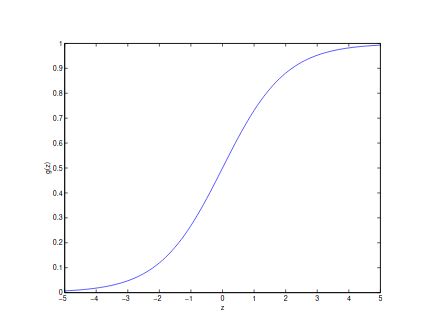
\includegraphics{images/sigmoid}
\end{figure}
For now, let’s take the choice of $g$ as given, in fact other functions that smoothly increase from $0$ to $1$
can also be used, but for a couple of reasons that we’ll see later, when we talk about GLMs, 
and when we talk about generative learning algorithms, the choice of the logistic function is a fairly natural one.

Before moving on, here’s a useful property of the derivative of the sigmoid function, which we write as $g'$
\begin{align*}
    g' & = \derivative{z} \frac{1}{1 + g^{-z}} \\
       & = \frac{1}{(1 + e^{-z})^2} (e^{-z}) \\
       & = \frac{1}{1 + e^{-z}} (1 - \frac{1}{1 + e^{-z}}) \\
       & = g(z) (1 - g(z)) 
\end{align*}
So, given the logistic regression model, to fit $\theta$ we follow how we saw least squares regression 
could be derived as the maximum likelihood estimator under a set of assumptions, let’s endow our 
classification model with a set of probabilistic assumptions, and then fit the parameters via maximum likelihood.

Let us assume that 
\begin{align*}
    P(y = 1 | x; \theta) & = h_{\theta}(x) \\
    P(y = 0 | x; \theta) & = 1 - h_{\theta}(x) \\
\end{align*}
Assuming that the $m$ training examples were generated independently, we can then write down the 
likelihood of the parameters as
\begin{align*}
    L(\theta) & = p(y | x; \theta) \\
              & = \prod _{i = 1}^m p(y^{(i)} | x^{(i)}; \theta) \\
              & = \prod _{i = 1}^m (h_{\theta}(x^{(i)}))^{y^{(i)}} (1 - h_{\theta}(x^{(i)}))^{1 - y^{(i)}} \\
\end{align*}
As before, it is more easy to maximise the log lihelikood 
\begin{align*}
    l(\theta) & = \log L(\theta) \\
              & = \prod _{i=1}^m y^{(i)} \log h_{\theta}(x^{(i)}) + (1 - y^{(i)}) \log (1 - h_{\theta}(x^{(i)})) \\
\end{align*}
Similar to our derivation in the case of linear regression, we can use \emph{gradient ascent} and 
written invectorial notation, our updates will therefore be given by
\[ \theta = \theta + \alpha \, \Delta _{\theta} \, l(\theta) \]
Let’s start by working with just one training example $(x, y)$, and take derivatives to derive
the stochastic gradient ascent rule
\begin{align*}
    \derivative{\theta_j} l(\theta) & = \left(y \frac{1}{g(\transpose{\theta} x)} - 
                                        (1 - y) \frac{1}{1 - g(\transpose{\theta} x)}\right) 
                                        \derivative{\theta_j} g(\transpose{\theta} x) \\
                                    & = \left(y \frac{1}{g(\transpose{\theta} x)} - 
                                        (1 - y) \frac{1}{1 - g(\transpose{\theta} x)}\right)
                                        g(\transpose{\theta} x)(1 - g(\transpose{\theta} x)
                                        \derivative{\theta_j} \transpose{\theta} x \\
                                    & = (y (1 - g(\transpose{\theta} x)) - (1-y) g(\transpose{\theta} x)) x_j \\
                                                 & = (y - h_{\theta}(x))x_j \\
\end{align*}
Above we used the fact that $g'(x) = g(x)(1-g(x))$ and therefore it gives us the stochastic gradient ascent rule
\[ \theta_j = \theta_j + \alpha (y - h_{\theta}(x))x_j \]
If we compare this to the LMS update rule, we see that it looks identical, but this is not 
the same algorithm, because $h_{\theta}(x^{(i)})$ is now defined as a non-linear function.\newline
Nonetheless, it’s a little surprising that we end up with the same update rule for a rather different algorithm
and learning problem, as how we will deeper talk in GLM(Generalized Linear Models) chapter.

\section{Perceptron algorithm}
We now digress to talk briefly about an algorithm that’s of some historical interest, 
and that we will also return to later when we talk about learning theory.\newline
Consider modifying the logistic regression method to “force” it to output values that are either $0$ or $1$.

To do so, it seems natural to change the definition of $g$ to be the threshold function

\[ g(z) = \begin{cases}
            1 \quad x \geq 0 \\
            0 \quad x < 0 \\
          \end{cases} \]

In the 1960s, this “perceptron” was argued to be a rough model for how individual neurons in the brain work and 
given how simple the algorithm is, it will also provide a starting point for our analysis when we talk
about learning theory later.

Note however that even though the perceptron maybe cosmetically similar to the other algorithms we talked about,
it is actually a very different type of algorithm than logistic regression and least squares linear regression;
in particular, it is difficult to endow the perceptron’s predictions with meaningful probabilistic interpretations,
or derive the perceptron as a maximum likelihood estimation algorithm.

